\section{Introduction}
Over the years, the amount of data we store and use has grown exponentially to the point that petabytes of storage is not uncommon. What used to be a simple task of accessing and sorting through information has been compounded into an arduous task with the size and scale of super-computing data centers. Being able to query data effectively, while also taking into account permissions becomes paramount into accomplishing daily tasks. This is what the Grand Unified File Index(GUFI) tool aims to accomplish. 
\\
\\
This process of efficiently accessing data is accomplished by recreating the tree structure via indexing. Each directory contains an SQL database file that stores the metadata of the files as well as summary information for that directory and optionally summary information for the entire tree below that directory. 

\begin{figure} [h]
\centering
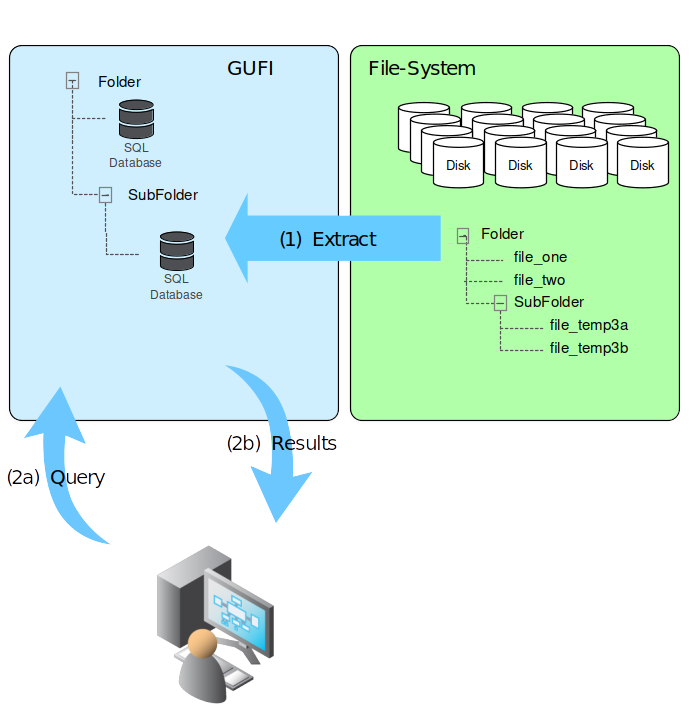
\includegraphics[width=0.5\textwidth]{images/gufi_structure.png}
\caption{\label{fig:gufi_structure}Layout and user interaction with GUFI}
\end{figure}
